\section{Testes de hipóteses}
\begin{frame}{Testes de hipóteses}
 \begin{itemize}
  \item Hipótese nula e alternativa;
  \item Hipóteses simples e compostas;
  \item Região crítica e estatística teste;
  \item Função poder;
  \item Tipos de erro (I e II);
  \item P-valor;
   \end{itemize}
\end{frame}

\begin{frame}{Hipótese nula e alternativa}
 No teste de hipóteses estatísticas, identificamos partições do espaço de parâmetros que codificam as hipóteses de interesse.
 \begin{defn}[Hipótese nula e hipótese alternativa]
  Considere o espaço de parâmetros $\Omega$ e defina $\Omega_0, \Omega_1 \subset \Omega$ de modo que $\Omega_0 \cup \Omega_1 = \Omega$ e $\Omega_0 \cap \Omega_1 = \emptyset$.
  Definimos
  \begin{align*}
   H_0 &:= \theta \in \Omega_0,\\
   H_1 &:= \theta \in \Omega_1.
  \end{align*}
Dizemos que $H_0$ é a~\textbf{hipótese nula} e $H_1$ é a~\textbf{hipótese alternativa}.

Se $\theta \in \Omega_1$, dizemos que~\textit{rejeitamos} a hipótese nula.
Por outro lado, se $\theta \in \Omega_0$ dizemos que~\textit{não rejeitamos} ou~\textit{falhamos em rejeitar} $H_0$.
 \end{defn}
\end{frame}

\begin{frame}{Exemplo}

Suponha que Palmirinha recebeu uma carta da Associação Nacional da Pamonha Gourmet (ANPG), dizendo que a pamonha deve ter, no mínimo, 7 mg/L de concentração de amido.
Supondo que a concentração de amido tenha distribuição Normal com parâmetros $\mu$ (desconhecido) e $\sigma^2$ (conhecido), Palmirinha rabisca num papel:
  \begin{align*}
   H_0 &:= \mu \in [7, \infty),\\
   H_1 &:= \mu \in (0, 7).
  \end{align*}
\end{frame}

\begin{frame}{Hipóteses simples e compostas}
 Dependendo do tipo de partição do espaço de parâmetros, as hipóteses recebem classificações diferentes.
 \begin{defn}[Hipótese simples e hipótese compostas]
  Dizemos que uma hipótese $H_i$, é~\textbf{simples}, se $\Omega_i = \{ \theta_i \}$, isto é, se a partição correspondente é um ponto. 
  Uma hipótese é dita~\textbf{composta} se não é simples.
 \end{defn}
 
 \begin{exemplo}[Hipótese simples sobre a média]
  Suponha que estamos estudando o efeito de uma droga na redução da pressão arterial.
  Modelamos esta redução como uma variável aleatória $X$ com esperança $E[X] =: \theta$.
  É costumaz testar a hipótese $H_0 : \theta = 0$, que chamamos, especificamente nesse caso, de ``hipótese de efeito nulo''.
 \end{exemplo}
\end{frame}

\begin{frame}{Hipótese unilateral e hipótese bilateral}
 Em analogia com os intervalos de confiança, também podemos entender as hipóteses como sendo unilaterais ou bilaterais.
 \begin{defn}[Hipótese unilateral e hipótese bilateral]
  Uma hipótese da forma $H_0 : \theta \leq \theta_0$ ou $H_0 : \theta \geq \theta_0$ é dita~\textit{unilateral} (``\textit{one-sided}''), enquanto hipóteses da forma $H_0 : \theta \neq \theta_0$ são ditas bilaterais (``\textit{two-sided}'').
 \end{defn}
 
 \begin{obs}[Hipóteses bilaterais como consequência de $H_0$ simples]
 Se $H_0$ é simples, a hipótese alternativa $H_1$ será, em geral, bilateral.  
 \end{obs}
\end{frame}

\begin{frame}{Região crítica: exemplo motivador}
 \begin{exemplo}[Teste para a média de uma Normal com variância conhecida]
  Suponha que $\bX = \{ \rs \}$ é uma amostra aleatória de uma Normal com média $\mu$ e variância $\sigma^2$ conhecida.
  Queremos testar a hipótese
  \begin{align*}
   H_0 &: \mu = \mu_0\\
   H_1 &: \mu \neq \mu_0.
  \end{align*}
  Intuitivamente, queremos rejeitar $H_0$ se $\Sm$ está longe de $\mu_0$.
  Para isso definimos
  \[ S_0 := \left\{ \bx: -c \leq \Sm - \mu_0 \leq c \right\}, \]
  de modo que $S_1 = S_0^C$. 
  Então, seguimos o procedimento:
      \begin{align*}
   \bX \in S_1 &\implies \text{rejeitar}\: H_0,\\
   \bX \in S_0 &\implies \text{não\:rejeitar}\: H_0.\\
  \end{align*}
 \end{exemplo}
\end{frame}

\begin{frame}{Região crítica e região de rejeição}
 Uma maneira mais simples de expressar o procedimento acima é definir $T := \left|\Sm - \mu_0\right|$ e rejeitar $H_0$ se $T \geq c$.
 \begin{defn}[Região crítica]
  O conjunto 
   \[ S_1 := \left\{ \bx:  \left|\Sm - \mu_0\right| \geq c \right\}, \]
   é chamado de~\textbf{região crítica} do teste.
 \end{defn}
 
Analogamente, considere a estatística $T = r(\bX)$ e tome $R \subseteq \mathbb{R}$. 
Então podemos definir
\begin{defn}[Região de rejeição]
Se $R \subseteq \mathbb{R}$ é tal que dizemos que ``rejeitamos $H_0$ se $T \in R$'', então $R$ é chamada uma~\textbf{região de rejeição} para a estatística $T$ e o teste associado.
\end{defn}
\end{frame}

\begin{frame}{Dividindo o espaço amostral e o espaço de parâmetros}
 Começamos com uma observação:
 \begin{obs}[Correspondência entre região crítica e região de rejeição]
 Podemos relacionar os conceitos de região crítica e região de rejeição notando queremos
   \[ S_1 := \left\{ \bx:  r(\bx) \in R \right\}. \]
\end{obs}

\begin{ideia}[Dividindo o espaço amostral e o espaço de parâmetros]
 Suponha que temos um modelo estatístico dado pela distribuição $f(x\mid\theta)$, com $x \in \mathcal{X}$ e $\theta \in \Omega$.
 Desta forma, uma amostra aleatória $\bX = \{ \rs\}$ mora em $\mathcal{X}^n$.
 Para formular uma hipótese estatística, estabelecemos uma partição do espaço de parâmetros $\Omega$ em $\Omega_0$ e $\Omega_1$ disjuntos.
 Isto, por sua vez, induz uma partição $S_0, S_1 \in \mathcal{X}^n$.
 Estes objetos, embora, relacionados,~\textbf{não são a mesma coisa}.
 Por exemplo, nós observamos se $\bX \in S_0$ ou $\bX \in S_1$, mas raramente ``observamos'' se $\theta \in \Omega_0$ ou $\theta \in \Omega_1$.
\end{ideia}
\end{frame}

\begin{frame}{Função poder}
 Nossa capacidade de rejeitar $H_0$ depende do valor de $\theta \in \Omega$.
 Esta dependência é capturada pela função poder.
 \begin{defn}[Função poder]
  Seja $\delta$ um procedimento de aceitação/rejeição como visto anteriormente.
  A~\textbf{função poder} é definida como 
  \begin{equation}
   \label{eq:power_function}
   \pi(\theta\mid \delta) := \pr\left(\bX \in S_1 \mid \theta\right) = \pr\left(T \in R \mid \theta\right), \theta \in \Omega.
  \end{equation}
 \end{defn}
Idealmente, queremos $\pi(\theta \mid \delta) = 1$ para $\theta \in \Omega_1$ (por quê?).
\end{frame}

\begin{frame}{A função poder de um teste para a média da Normal}
 Considere a situação em que $\rs$ vêm de uma Normal com média $\mu$, desconhecida, e variância $\sigma^2$, conhecida.
 \begin{exemplo}[Função poder no teste para média da Normal ($\sigma^2$ conhecida)]
  Lembrando que $T = |\Sm - \mu_0|$, e tomando $\delta$ como o procedimento descrito acima, escrevemos
  \begin{align*}
   \pi(\mu \mid \delta) &= \pr(T \in R \mid \mu),\\
   &= \pr\left(\Sm \geq \mu_0 + c \mid \mu \right) + \pr\left( \Sm \leq \mu_0 -c \mid \mu \right),\\
   &= \left\{ 1 - \Phi\left(\sqrt{n} \frac{\mu_0 + c -\mu}{\sigma}\right) \right\} + \Phi\left(\sqrt{n} \frac{\mu_0 - c -\mu}{\sigma}\right). 
  \end{align*}
 \end{exemplo}
\end{frame}

\begin{frame}{Pelo poder da pamonha...}
\begin{figure}
 \begin{center}
  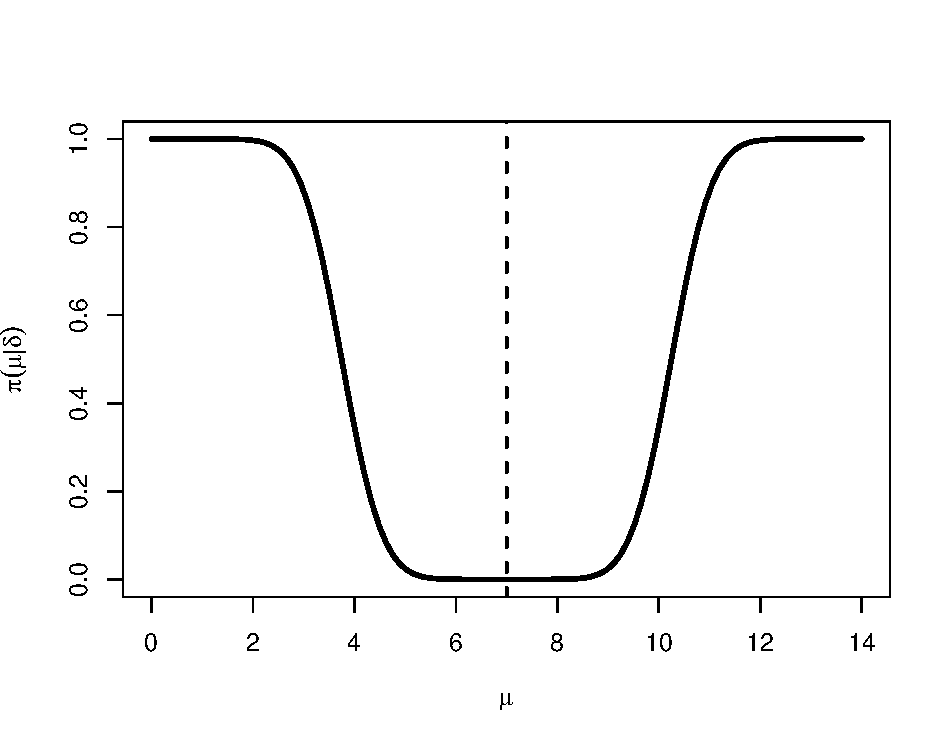
\includegraphics[scale=0.6]{figures/poder_palmirinha.pdf}
 \end{center}
\end{figure} 
\end{frame}
 
\begin{frame}{Tipos de Erro}
 Quando testamos uma hipótese, nunca estamos livres de cometer um erro.
 É conveniente classificar os possíveis erros em duas categorias.
 \begin{defn}[Tipos de erros]
 \begin{center}
  \begin{tabular}{cc}
   Nome & Erro cometido\\
   \hline
   Erro tipo I & Rejeitar $H_0$ quando ela é~\textbf{verdadeira}.\\
   Erro tipo II & Falhar em rejeitar $H_0$ quando ela é~\textbf{falsa}.\\
   \hline
  \end{tabular}
 \end{center}  
 \end{defn}
Isto nos leva a concluir que
\begin{center}
  \begin{tabular}{ccl}
   Situação & Quantidade & Interpretação\\
   \hline
    $\theta \in \Omega_0$ & $\pi(\theta \mid \delta)$ & $\pr(\text{Erro\: tipo\: I})$ \\
    $\theta \in \Omega_1$ & $1-\pi(\theta \mid \delta)$& $\pr(\text{Erro\: tipo\: II})$\\
   \hline
  \end{tabular}
\end{center} 
 \end{frame}

\begin{frame}{Balanceando um teste}
 Idealmente, gostaríamos de um teste $\delta$ para o qual as probabilidades de erro fossem as menores possíveis. 
 Infelizmente, em geral, diminuir o erro tipo I implica aumentar o erro tipo II. 
%  Tome, por exemplo, um teste $\delta_0$ que~\textbf{nunca} rejeita $H_0$, terá $\pi(\theta \mid \delta_0 = 0$ para todo $\theta \in \Omega_0$, o que é bom, mas também terá  $\pi(\theta \mid \delta_0 = 0$ para $\theta \in \Omega_1$, o que é bem ruim.

 Em geral, precisamos encontrar um equilíbrio entre os tipos de erros.
 \begin{ideia}[Encontrando um balanço entre erro tipo I e tipo II]
  Tome $0 < \alpha_0 < 1$.
  Nós construímos o procedimento $\delta^\ast$ de modo que
  \begin{equation}
  \label{eq:test_maxsize}
   \pi(\theta \mid \delta^\ast) \leq \alpha_0, \: \forall\: \theta \in \Omega.
  \end{equation}
 Então, entre todos os testes que satisfazem~(\ref{eq:test_maxsize}), buscamos o teste que tenha $\pi(\theta \mid \delta^\ast)$ máxima em $\theta \in \Omega_1$.
 \end{ideia}
\end{frame}
 
 
\begin{frame}{Tamanho de um teste}
 \begin{defn}[Tamanho/nível de um teste]
 Dizemos que um teste, $\delta$, tem~\textbf{tamanho} ou~\textbf{nível de significância} $\alpha(\delta)$, com 
 \begin{equation*}
  \alpha(\delta) := \sup_{\theta \in \Omega_0} \pi(\theta \mid \delta).
 \end{equation*}
 \end{defn}
Um teste que atende à condição anterior (\ref{eq:test_maxsize}) tem que tamanho?

\begin{obs}[Tamanho de um teste com $H_0$ simples]
 Se $H_0$ é simples, então $\alpha(\delta) = \pi(\theta_0 \mid \delta)$.
\end{obs}

\end{frame}

\begin{frame}{Um exemplo}
 \begin{exemplo}[Teste para o parâmetro de uma uniforme]
  Suponha que $\rs$ tem distribuição Uniforme em $[0, \theta]$, com $\theta$ desconhecido, e que aventamos as seguintes hipóteses:
  \begin{align*}
   H_0:&\: 3 \leq \theta \leq 4, \\
   H_1:&\:  \theta < 3 \:\text{ou}\: \theta > 4
  \end{align*}
  Lembre que $\emv = \max\{\rs\}$ e suponha que temos um teste $\delta$ da forma  
   \begin{center}
  \begin{tabular}{cc}
   Condição & Ação \\
   \hline
   $\emv \notin (2.9, 4)$ & Rejeitar $H_0$ \\
   $\emv \in (2.9, 4)$ & Falhar em rejeitar $H_0$.\\
   \hline
  \end{tabular}
 \end{center}  
 \end{exemplo}
\begin{itemize}
 \item Qual a região de rejeição para $\delta$?
 \item Como escrever $\pi(\theta \mid \delta)$?
 \item Qual o tamanho de $\delta$?
\end{itemize}
\end{frame}

\begin{frame}{Construindo um teste com o tamanho adequado}
 Em geral, sempre conseguimos construir um teste que tenha o tamanho desejado.
 \begin{obs}[Construindo um teste de tamanho $\alpha_0$]
  Se $T = r(\bX)$ é uma estatística, podemos quase sempre encontrar $c$ tal que valha
  \begin{equation}
   \label{eq:size_test_statistic}
   \sup_{\theta \in \Omega_0} \pr\left(T \geq c \mid \theta \right) \leq \alpha_0,
  \end{equation}
  ou seja, encontrar $c$ tal que $\delta$ tenha tamanho (ou nível de significância) $\alpha_0$.
 \end{obs}
\end{frame}

\begin{frame}{O p-valor}
Começamos com uma observação:
\begin{obs}[Testes são decisões binárias]
 Um teste de hipótese reduz a informação contida nos dados a uma decisão binária: rejeitar ou não $H_0$. 
 Se observamos $T = c + 10^{-10}$ ou $T = c + 10^{10}$, tomamos a~\textit{mesma decisão} de rejeitar $H_0$ ao nível $\alpha_0$.
\end{obs} 
Ao invés disso, podemos reportar o maior nível de significância que ainda levaria à rejeição de $H_0$.
\begin{defn}[O p-valor]
 \label{def:pvalue}
 Para cada $t$, seja $\delta_t$ o teste que rejeita $H_0$ se $T \geq t$.
 Então, quando $T = t$, o~\textbf{p-valor} vale
 \begin{equation}
   p(t) := \sup_{\theta \in \Omega_0} \pi(\theta \mid \delta_t) = \sup_{\theta \in \Omega_0} \pr\left(T \geq t \mid \theta \right),
 \end{equation}
ou seja, o p-valor é o tamanho do teste $\delta_t$.
\end{defn}
\end{frame}

\begin{frame}{Exemplo: tá me enganando, parceiro?}
Vamos voltar a uma pergunta não respondida lá no início do curso.
Suponha que você encontre um ``artista'' de rua, que joga uma moeda e pede para as pessoas apostarem se vai dar cara ou coroa.
Conhencendo estatística e probabilidade, você decide (i) observar o jogo à distância para coletar alguns dados (ii) fazer algumas contas para ver se vale a pena apostar.
 \begin{pergunta}[Esta moeda é justa? cont. I]
 \label{ex:moeda_justa_reborn}
  Suponha que uma moeda tenha sido lançada dez vezes, obtendo o seguinte resultado:
  \begin{equation*}
   KKKCKCCCKC
  \end{equation*}
\begin{itemize}
 \item[a)] Esta moeda é justa?
 \item[b)] Quanto eu espero ganhar se apostar R\$ 100,00 que é justa? 
\end{itemize}
 \end{pergunta}
 Hoje vamos dar uma resposta parcial à pergunta a).
\end{frame}

\begin{frame}{O que aprendemos?}
\begin{itemize}

  \item[\faLightbulbO] Hipóteses nula e alternativa, simples e composta;    
  \item[\faLightbulbO] Região crítica e região de rejeição;
  \item[\faLightbulbO] Função poder;
  
  ``O poder de um teste é a probabilidade de rejeitarmos $H_0$ caso ela seja falsa''
  
  \item[\faLightbulbO] Erro tipo I e tipo II;
  \begin{itemize}
   \item Tipo I: Rejeitar erroneamente $H_0$;
   \item Tipo II: Falhar em rejeitar $H_0$ quando ela é falsa.
  \end{itemize}
  \item[\faLightbulbO] P-valor;
  
  ``O p-valor pode ser interpretado como a probabilidade, sob $H_0$, de observarmos uma estatística tão ou mais extrema do que aquela observada''
  \end{itemize}
 \end{frame}

\begin{frame}{Leitura recomendada}
\begin{itemize}
 \item[\faBook] De Groot seção 9.1;
 \item[\faBook] $^\ast$ De Groot seções 9.2 e 9.3.
%  \item[\faBook] $^\ast$ Schervish (1995), capítulo 7.
%  \item[\faBook] $^\ast$ Casella \& Berger (2002), seção 9.2.
 \item[\faForward] Próxima aula: De Groot, seção 9.1 (razão de verossimilhanças);
 \item {\large\textbf{Exercícios recomendados}}
 \begin{itemize}
  \item[\faBookmark] De Groot.
  \begin{itemize}
   \item Seção 9.1: 3, 8 e 13.
   \item $^\ast$ Seção 9.1: 19 e 21.
  \end{itemize}   
  \end{itemize}
 \end{itemize} 
\end{frame}
